\chapter{Concept}
In the previous \textbf{\nameref{2_relatedWork}} and the \textbf{\nameref{3_slacklining}} chapter is described how other applications realized similar application with other activities, what slacklining in particular is and which learning techniques exist to learn and master it. Mostly this is done with a professional who already knows how to act on the line and where particular attention must be paid. In contrast to such a human personal trainer this thesis will elaborate an interactive slackline learning system with real-time feedback. The idea of this system is, that the user can learn slacklining only with the given application. One main feature is that it should be an autonomous system. This gives the opportunity to be independent of other human help and therefore it can only 
be controlled by the by the user that is currently interacting with the system. To help her with exercise execution it responds to the actions of the user and provides him with feedback such that the user can correct himself. To built such a system a concept has to be built, which is part of this chapter. Therefore in the following a conceptual analysis will be elaborated. It involves \textbf{\nameref{4_2_general}} where basic requirements of the entire system are described. This is followed by the more specific sections \textbf{\nameref{4_2_interaction}}, \textbf{\nameref{4_3_stages}} and \textbf{\nameref{4_4_exercises}} as well as \textbf{\nameref{4_5_feedbackSystem}}, which describes how feedback is properly given to the user. Lastly the section \textbf{\nameref{4_6_scenario}} gives a better overview about the worflow of the particular components and \textbf{\nameref{4_7_conclusion}} will wrap up of each part of the concept.
\section{General Information}\label{4_1_general}
In general the system should be easy to understand, to learn, and to interact. To achieve this it should provide proper user experience. Usability heuristics are useful to identify or to prevent problems in a system. Therefore the system will rely on the interaction design principles by Nielsen~\cite{Nielsen_1994-he} described in section \textit{\nameref{nielsenDesignPrinciples}}. Beside this certain tasks have to be considered that are more related to this system. An overview about these can be found in section \textit{\nameref{systemBasics}}.

\subsection{Ten heuristic principles for interaction design}\label{nielsenDesignPrinciples}
Nielsen designed his ten heuristics by comparing several sets of usability heuristics with existing usability problems from certain projects~\cite{Nielsen_1994-he}. Hence he was able to determine what heuristics identify usability problems the best and therefore creating a set of them. To prevent that a system results in having such problems they can also be used as a guideline for designing and developing a user friendly system. The interactive slackline system will follow these principles, which are described in the following:

\textbf{\hyperref[4_1_1_visibilitySystemStatus]{Visibility of system status}}\\
The system should always keep the user informed about the current state through appropriate feedback in an adequate time.\\

\textbf{Match between system and the real world}\\
The system should provide the user with familiar terms and information. Using technical terms with which she is not familiar can lead to confusion. Therefore proper information should be natural and in a meaningful order.\\

\textbf{User control and freedom}\\
If the user clicks accidently on something she should be able to leave this state without any troubles.\\

\textbf{Consistency and standards}\\
It should follow a clear design standard and provide consistency. The user should not be confused whether different terms or elements mean the same.\\

\textbf{Error prevention}\\
Conditions and actions that could easily result in errors should be prevented. Another option is to inform the user about the consequences that the action may have and which she has to actively confirm.\\

\textbf{Recognition rather than recall}\\
The users memory load has to be minimized. She should not remember every action or information. Elements, actions, and options should be visible and instructions about the usage must be easy to retrieve.\\

\textbf{Flexibility and efficiency of use}\\
Providing quick options and allowing to skip certain steps can speed up the interaction for more familiar users. Hence the system should take care of both novice and experienced users.\\

\textbf{Aesthetic and minimalistic design}\\
Information should just contain aspects that are relevant to the user and that she really needs. Every irrelevant data decreases the intelligibility.\\

\textbf{Help users recognize, diagnose, and recover from errors}\\
Error messages should accurately indicate the ongoing problem such that the user knows what is wrong. Providing a constructive solution helps the user to solve the problem.\\

\textbf{Help and documentation}\\
Optimally the system can be used without any further documentation. It may be the case to provide help and documentation. If it cannot be circumvented it should be easy to find it and clearly show the relevant steps.\\

\subsection{System specific basics}\label{systemBasics}
One person at a time should be able to interact with the system. This is because mostly just one person can stay on the slackline especially for beginners. However it should provide the ability to have multiple user profiles. One can switch between those such that several persons can have a profile on the same application. For proper user training the system should follow a clear workflow. Therefore two methods have been discussed in section \textit{\nameref{3_3_1_learningConcepts}}. A methodical routine will be used with which stages and exercises can be designed as levels. These should be locked at the beginning and the user can unlock them by successfully executing the prior exercise. Another important part is the user tracking. The system should be able to track the user in an appropriate accuracy and precision such that it can match the users movement with the actual exercise. This is in correlation with properly providing real-time feedback, which is further discussed in section \textit{\nameref{4_5_feedbackSystem}}. All relevant recorded data should be immediately saved when it is needed, e.g. when successfully accomplishing an exercise.

\begin{comment}
- System should be able to track user appropriately
- All relevant data should be immediately saved when it is needed (unlocking exercise/stage, failing/accomplish exercise)
- Information about where the user currently is should be given --> title
- User selection
- Also a possibility to go to the last screen if she misclicks should be given.
\end{comment}
\section{Interaction}\label{4_2_interaction}
A bigger part of the system is the interaction since it is independent of any external controlling devices.
The user should be able to navigate through the system by herself with her hands as interaction input.
A cursor should always be visualized to navigate through the systems interface.
If the user initially starts the system, there should be an engagement gesture to convey that the system initially recognises and responds to a user action.
Furthermore, a small tutorial should be given in which the user will be trained on how to use the interaction possibilities with the system (\textit{cf. \hyperref[nielsenDesignPrinciples]{Recognition rather than recall}}).
To make her familiar with these, she should directly apply these techniques in the tutorial.
The current state of the interaction is clearly visualized, such that the user knows if she triggers an action regarding an element (\textit{cf .\hyperref[nielsenDesignPrinciples]{Visibility of system status}}).
To be able to interact with elements and start the exercise execution the user should stay in a predefined initial position.
The SLS then recognises if a user is ready to start. Interaction will also play a role in exercise execution.
During the execution she interacts with the SLS by trying to match the predefined exercise.
The user should then get appropriate feedback, which is further explained in section \textit{\nameref{4_5_feedbackSystem}}.

\begin{comment}
- user can and should interact with the system
\\- Cursor visualization as hand image
\\- Engagement gesture for first interaction with Kinect (One hand over shoulder)
\\- She should be instructed how to interact 
\\- Different interaction methods should be provided to prevent failing on one (tutorial --> clicking (variations) + scrolling)
\end{comment}
\section{Stages}\label{4_3_stages}
The system covers predefined gestures, which are subdivided in stages that have been elaborated in subsection \textit{\nameref{3_3_2_StagesExercises}}. Since the interactive slackline system follows a slightly exergame like approach, the stages and exercises should be designed as levels, which the user could select has to unlock. Therefore a menu should exist for all available stages as well as for all exercises within a stage. To give her a starting position, the very first stage and exercise should be interactable. 
She can then unlock the next stage by accomplishing all exercises in the last one. Hence it can be assured that the user is able to encounter with the more difficult exercises. She should also be introduce in each stage to know how its purpose and goal. At last a summary can be given to show an overview of her performance for the entire stage.

%The user should also be introduce in each exercise to know how to perform it correctly and give her support for successfully executing it

\section{Exercises}\label{4_4_exercises}
%should have predefined exercises that can be tracked in an appropriate manner
Each exercise is part of one stage. It is divided into two body sides, which consists of several repetitions (Figure \ref{fig:exerciseStructure}). Every exercise is locked except the first one to provide a starting point, like with the stages. The next exercise should be unlocked by accomplishing both sides of the current one. Similarly a side will be completed if all repetitions have been finished. Like for the stage, each exercise should be instructed for the user such that she can successfully perform it. The system will also recognise if the user is ready to start with the exercise. During the execution she should get real time feedback about her current performance. An exercise summary should then show the performance of the execution with several performance parameters regarding the given exercise.

\begin{figure}[htb]
	\centering
	\begin{minipage}[t]{1\linewidth}
		\centering
		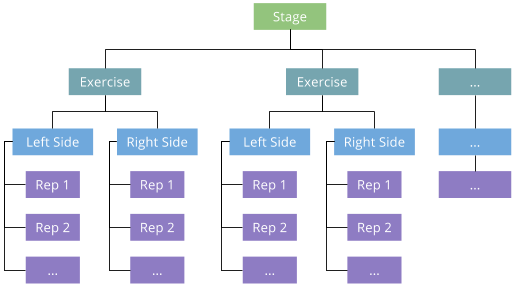
\includegraphics[width=1\linewidth]{Pictures/exerciseStructureTopDown2}
		\caption{Exercise structure}
		\label{fig:exerciseStructure}
	\end{minipage}
\end{figure}
\begin{comment}
\\- system should provide predefined exercises that can be tracked per user
\\- A stage menu should be provided to the user, which shows her the amount of stages to complete
\\- It consists of 4 stages each with specific exercises (Preliminary, First contact with slacklining,  Static exercises, Dynamic exercises) like explained in chapter 3
\\- A stage consists of several exercises like explained in prev. chapter
\\- locked stages (initial first stage interactable)
\\- unlock stages (by successfully accomplishing all exercises from current stage)
\\- Stage introduction gives general information, describes the goal and tips for the current stage
-- a stage information scene provides her with the general introduction of this stage --> unlocks first exercise
\\- Stage summary contains average data about each exercise
\end{comment}

\section{Feedback system}\label{4_5_feedbackSystem}
%The user should get feedback about her performance during exercise execution. 
%Another big role of this plays in the exercise execution. Here the user interacts with the system to match a predefined gesture for accomplishing the exercise. Therefore real time feedback is provided which gives her hints about the right interaction and how good it is performed. More information about the feedback methods can be found in feedback system

% - https://www.researchgate.net/profile/Eduardo_Velloso/publication/262162999_MotionMA_Motion_modelling_and_analysis_by_demonstration/links/577a4aaa08aece6c20fbc5bf.pdf
% - https://www.ncbi.nlm.nih.gov/pubmed/27555917
% - http://online.liebertpub.com/doi/abs/10.1089/g4h.2012.0041?url_ver=Z39.88-2003&rfr_id=ori%3Arid%3Acrossref.org&rfr_dat=cr_pub%3Dpubmed&
% - https://www.ncbi.nlm.nih.gov/pmc/articles/PMC4835340/
% - http://ieeexplore.ieee.org/document/7399879/

% - https://www.akqa.com/work/nike/kinect/
% - https://www.ea.com/de-de/news/ea-sports-active-2-bringt-fitnessfans-in-die-form-ihres-lebens

Feedback is the main and most powerful component of the interactive learning system. Since the user should interact on her own with the system one has to assume that no other person interfere with her and the system. With this in mind the feedback of the system should designed in a way, that the user knows at any time what she has to do or has done. In general audio and visual feedback will be provided to the user. Regarding the \textbf{\nameref{4_2_interaction}} with the system, e.g. clicking a button, the system should respond with an audio signal and change the elements visual state accordingly.

For the accomplishment of the exercise execution it is essential to provide real-time feedback. This supports her during the performance and enhances the learning effect more than with post feedback methods, like discussed in \textbf{\nameref{2_3_3_feedbackApproachesTechniques}}. Hence the overall exercise execution can be improved by providing appropriate real-time feedback. The system should therefore response to the user like seen in other applications \textbf{\todo{[cite, maybe Related Work --> Nike + / EA SPORTS Active 2]}}. These responses should mainly contain an indicator if the execution is currently performed right or not, visualize the the performance of the user regarding the predefined gestures, and the progress of the the current execution. The user should also see herself mirrored in an appropriate environment to know how the executes the exercises and if she is in detection range of the kinect sensor. With this a baseline is built for appropriate real time feedback to the user.

\begin{comment}
- in general audio and visual feedback
- if the user has clicked a button
- stays in the right position
- Indicator about if exercise is correctly executed
- Indicator about how good the exercise is performed
- real time feedback (Time, confidence, checklist, repetitions)
- system should inform how many repetitions are left
- system should inform when the repetition is successfully accomplished (audio, visual -> timer green, repetition counter)
- system should inform the user if repetition was not successful (audio, visual -> reset timer, checklist)
- After successful execution, a summary is shown about the performance of the user for each rep (time, attempts, confidence)
- tier summary (avg. time, attempts, confidence)
\end{comment}

%\section{Scenario}\label{4_6_scenario}
%To have a better understanding regarding the interplay of the several components a generic scenario workflow will be given from a users' point of view. The users' name is Bob and he is 21 years old. While climbing with friends in a climbing hall he noticed a new interactive learning system that they provide to visitors for trying and learning slacklining. He heard once of this activity by friends but never had the chance to try it. So he decides to test it and wants to execute some exercises. To engage with the system he has to stay in front of it, which recognizes him immediately. At the beginning it introduces him regarding the interaction possibilities. After that, he selects a tier and is further informed about the goal and basics of this stage. Once confirming that he read everything it leads him to the first available exercise. The system shows him how to execute it properly. Right after starting the exercise he gets helpful real time feedback to correct himself for a successful accomplishment of the execution. After finishing the exercise Bob gets an overview about his performance.

%asks him to do an engagement gesture. Now he is introduced in the interaction of the system. After he knows how to interact with the system he can select a user profile, which was created by the personal before. This will lead him to the stage selection. He selects the very first because all others are locked. In here bob has to read the instructions for the stage to be informed about what he has to pay attention for. Next he selects the first exercise and a body side he wants to train. Before bob can start with the execution, he will be informed about how this specific exercise is executed and how to perform it. After he thinks that he is ready to challenge it, he starts the exercise explicitly. Now he sees all relevant information about the execution and starts to execute it. He notices that the system gives him real time feedback about his performance and the progress made. After finishing all repetition the system leads him to the exercise summary screen, which gives an overview about the performance of the just executed exercise. 

%The user raises the hands over her head to start the application. She is now instructed on how to interact with elements on  the screen, e.g. clicking and scrolling. After being confident with this, she selects her user profile to load the appropriate exercises and leads her to the stage selection. She selects the first stage since all others are currently locked. Now she is in the exercise menu. In here she clicks on the \textit{stage information} button, which gives her an introduction into the stage. After confirming that she has read the introduction the first exercise becomes unlocked and she selects it. After that she decides to train her left leg first in the side selection. An exercise introduction screen is following, which shows specific information about the execution. After reading the introduction she feels ready to counter the exercise. Therefore she goes into the starting position and starts the exercise by clicking the start button.

%The screen changes and all relevant elements are shown for the exercise execution. She performs every repetition of the exercise successfully. After finishing these the system leads her to the exercise summary screen, which shows her the performance of the just executed exercise. In here she can now decide to return to the main menu or go on and start the training for the other body side. This procedure is also visualized in Figure \ref{fig:scenarioWorkflow} below.

\section{Conclusion}\label{4_7_conclusion}